% ---------------------------------------------------------------
% Esbocos gerados por desenhos/esboco.py - cole onde couber.
% Os PDFs ficam em desenhos/. No Overleaf, o \graphicspath do
% preambulo ja aponta para imagens/, entao ou copie os PDFs para
% imagens/ ou use o caminho completo, como abaixo.
% ---------------------------------------------------------------

\begin{figure}[h!]
    \centering
    \caption{Esboco inicial do produto: vistas, detalhe do mecanismo e fluxo de uso}
    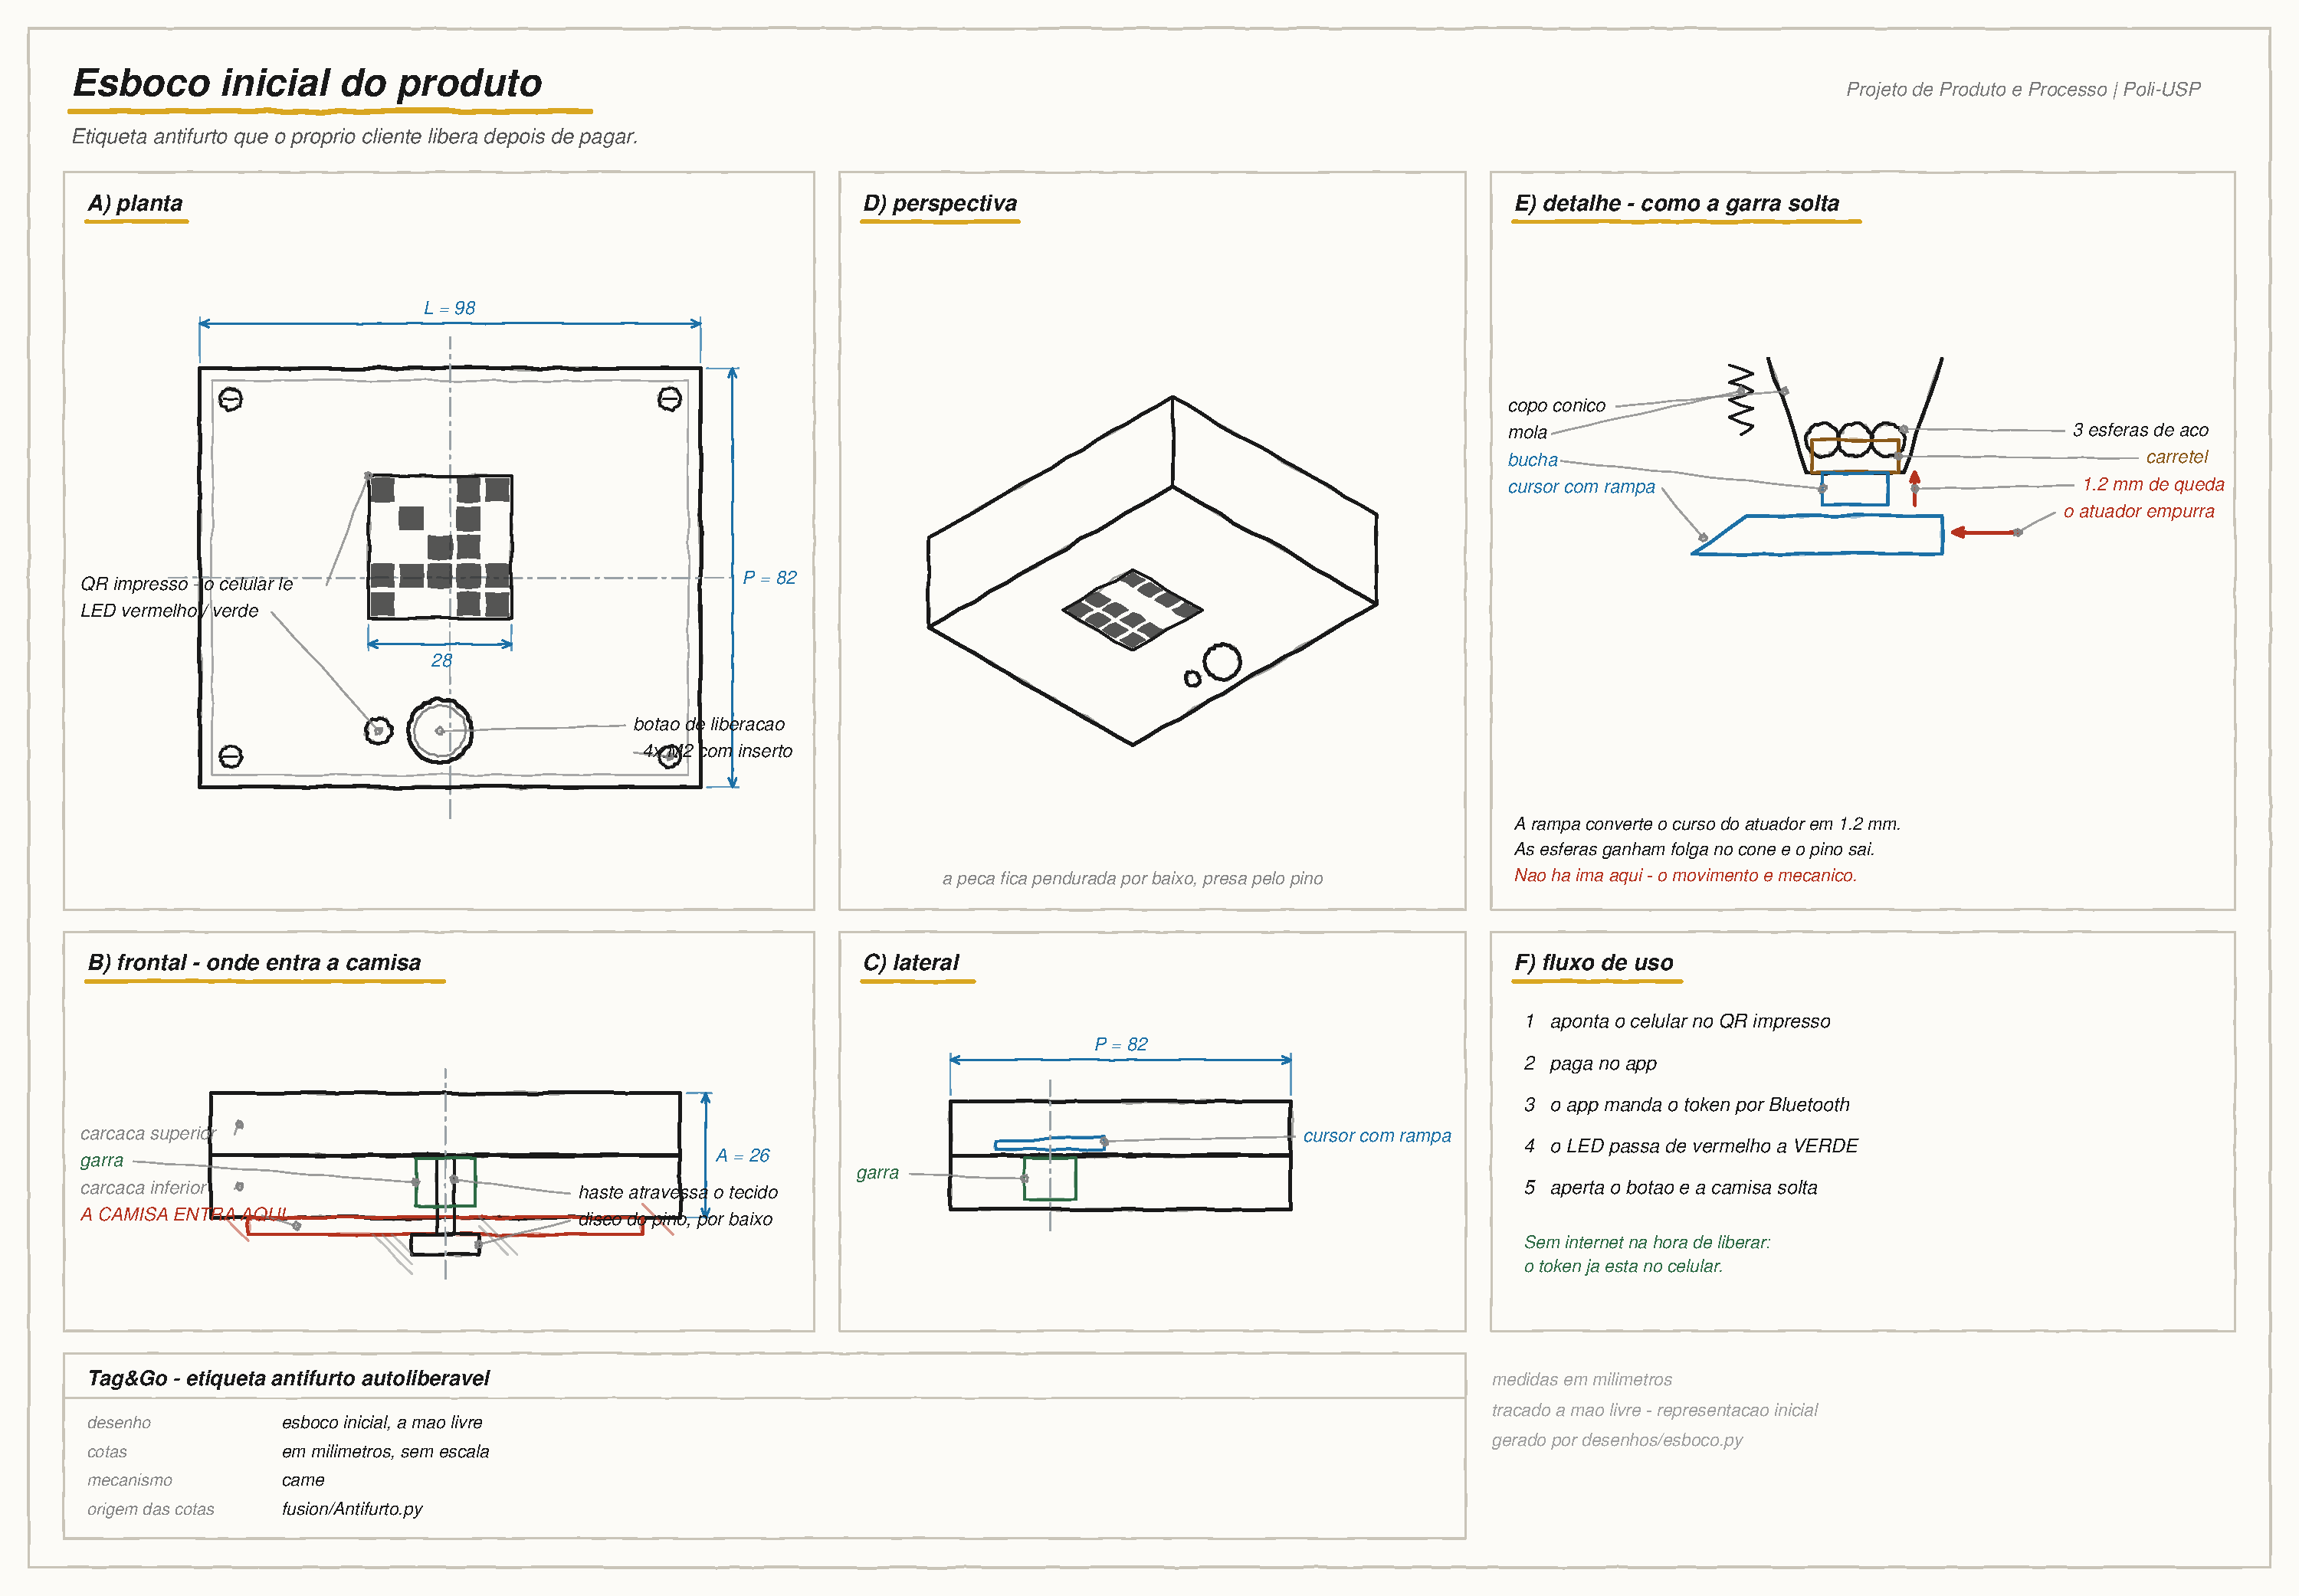
\includegraphics[width=\textwidth]{desenhos/esboco.pdf}
    \label{fig:proposta-esboco-geral}
    \source{Autor}
\end{figure}

\begin{figure}[h!]
    \caption{Vistas do dispositivo}
    \begin{subfigure}{0.48\textwidth}
        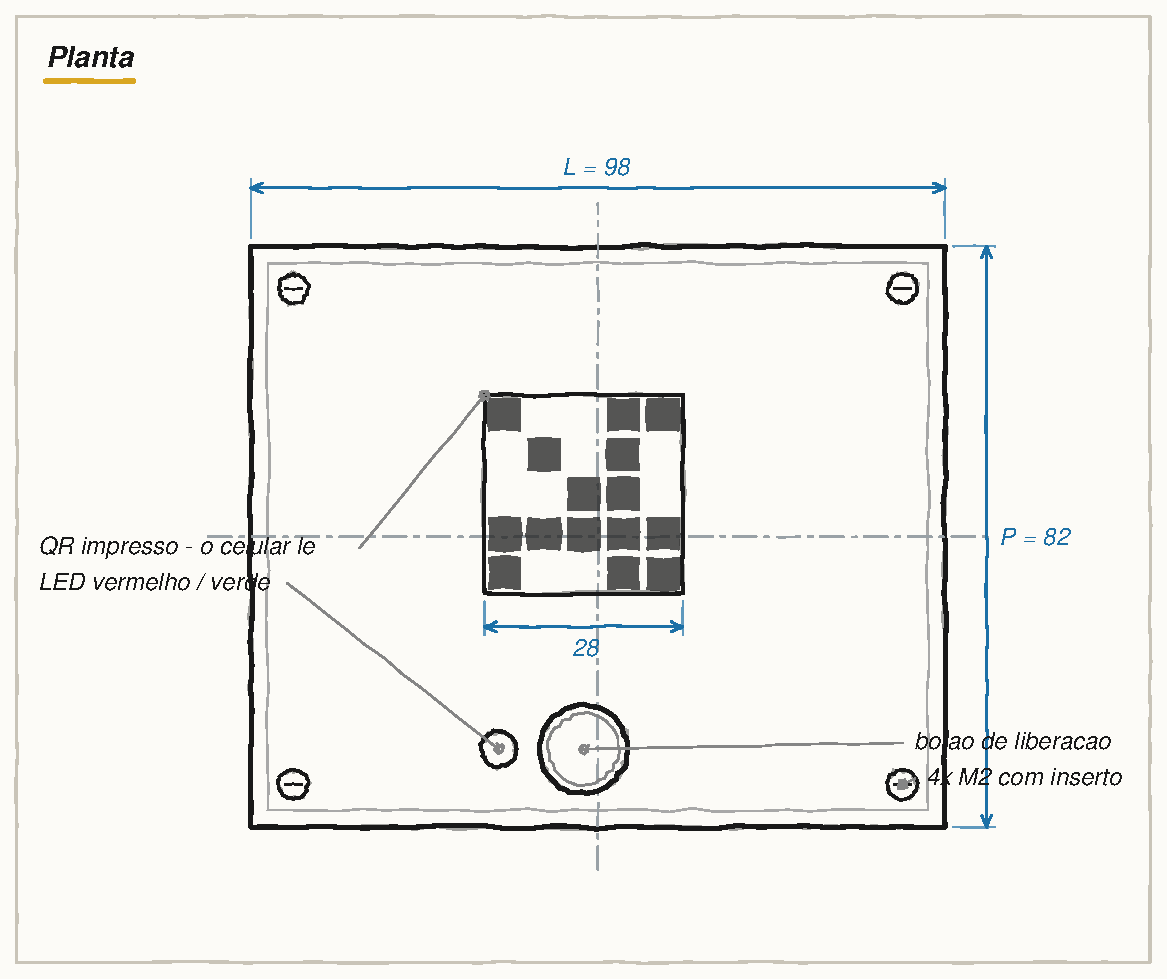
\includegraphics[width=0.95\textwidth]{desenhos/fig-planta.pdf}
        \caption{Planta}
        \label{fig:proposta-planta}
    \end{subfigure}%
    \begin{subfigure}{0.48\textwidth}
        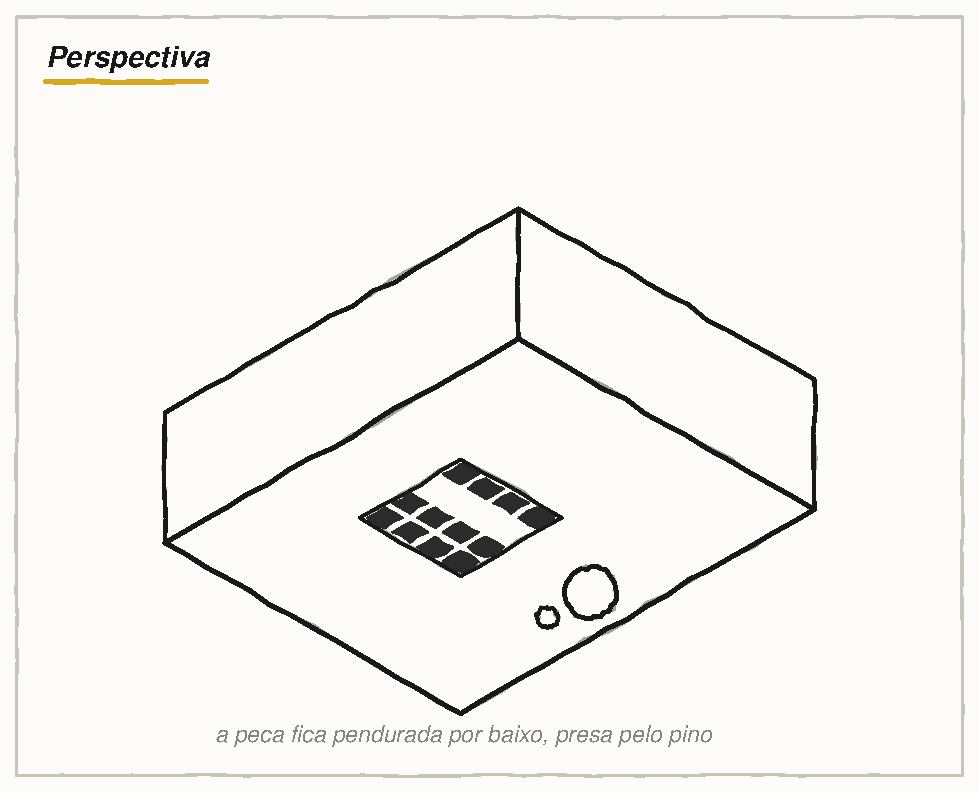
\includegraphics[width=0.95\textwidth]{desenhos/fig-perspectiva.pdf}
        \caption{Perspectiva}
        \label{fig:proposta-perspectiva}
    \end{subfigure}
    \begin{subfigure}{0.48\textwidth}
        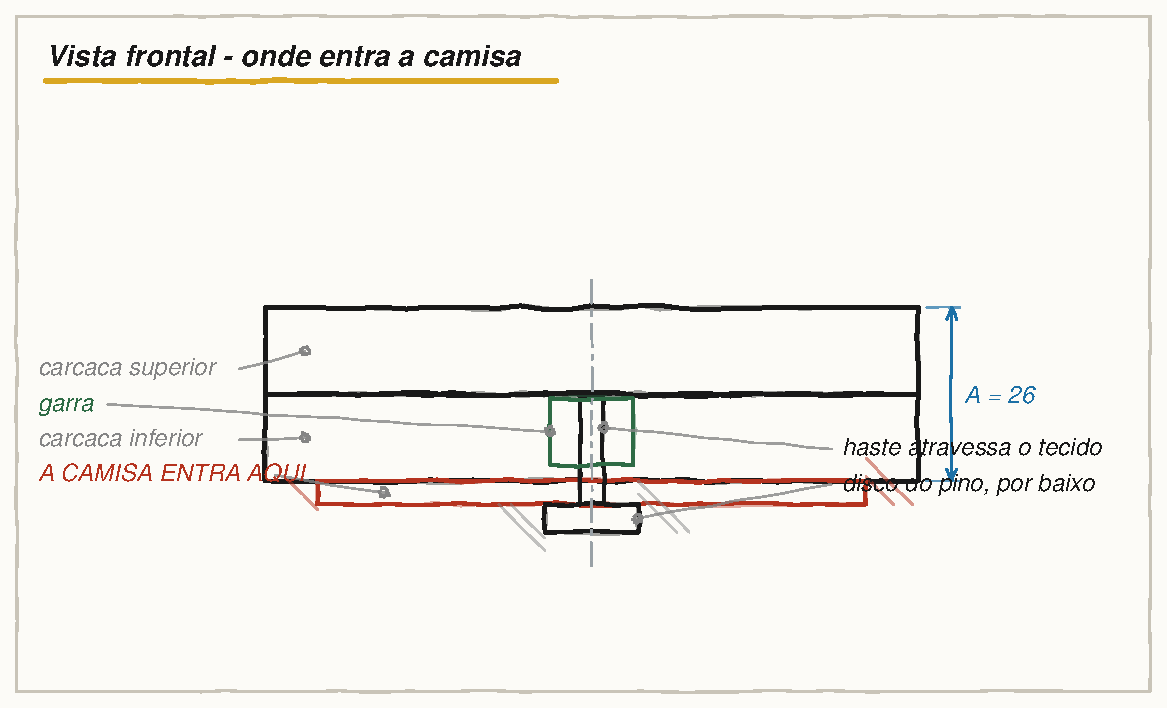
\includegraphics[width=0.95\textwidth]{desenhos/fig-frontal.pdf}
        \caption{Vista frontal, mostrando onde a peca de roupa e presa}
        \label{fig:proposta-frontal}
    \end{subfigure}%
    \begin{subfigure}{0.48\textwidth}
        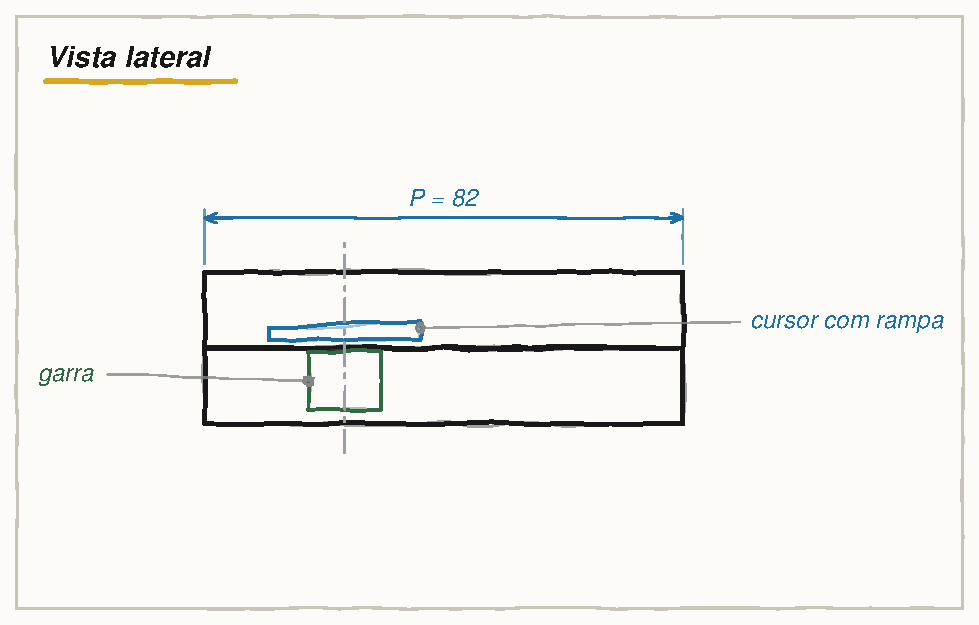
\includegraphics[width=0.95\textwidth]{desenhos/fig-lateral.pdf}
        \caption{Vista lateral}
        \label{fig:proposta-lateral}
    \end{subfigure}
    \label{fig:proposta-vistas}
    \source{Autor}
\end{figure}

\begin{figure}[h!]
    \centering
    \caption{Detalhe do mecanismo de destravamento}
    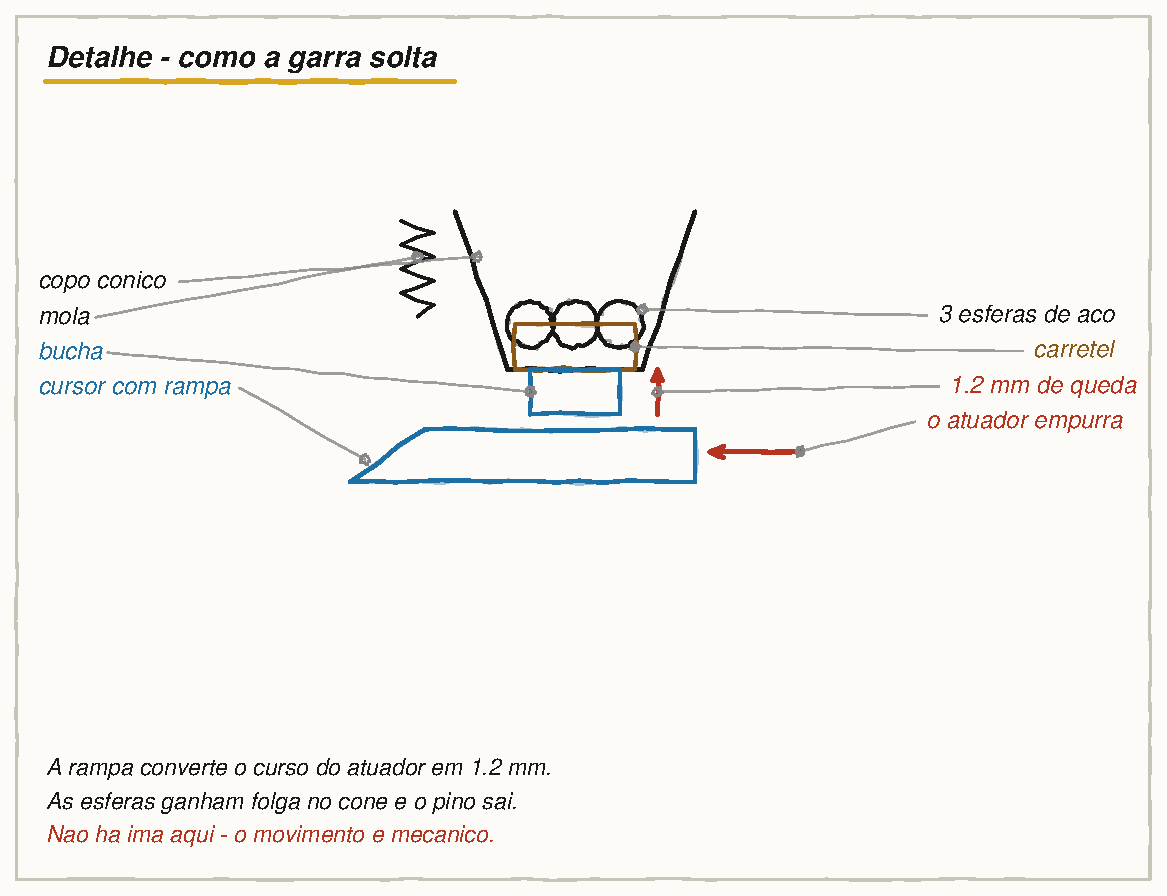
\includegraphics[width=0.8\textwidth]{desenhos/fig-detalhe.pdf}
    \label{fig:proposta-detalhe}
    \source{Autor}
\end{figure}
